\section{Data protection and the GDPR}
\subsection{Article 8 (Not GDPR)}
Article 8 can be summarized in three main points:
\begin{enumerate}
  \item Everyone has the right to protection of personal data concerning him or her.
  \item Such data must be processed fairly for specified purposes and on the basis of the consent of the person concerned or some other legitimate basis laid down by law. Everyone has the right of access to data which has been collected concerning him or her, and the right to have it rectified.
  \item Compliance with these rules shall be subject to control by independent authority.
\end{enumerate}
This is one of the most important articles because in the first point we assume that all our data must be protected.
In the second point, instead, we say that personal data can be used only for a specific purpose, so how we will see after, if we collect data for a specific purpose we can't use them for another analysis.
\subsection{Main pillars}
Generally speaking, there are six key elements common to all the data protection legislation that came over the years and in different european countries:
\begin{enumerate}
    \item \textbf{Data-centric model}: personal data is the most important asset discussed; all the regulations are about user data and their processing and they do not depend on the infrastructure.
    \item \textbf{Tech neutral approach}: there is no need to explain technology used but give principle of accountability (explain decisions you make by a tech point of view)
    \item \textbf{Legal basis}: the general approach is that you can process data only if there is a specific legal basis to do so.
    \item \textbf{Procedural approach}: not strictly legal. Specific procedures for each situation (collection, handling, etc…)
    \item \textbf{Risk management}: when you make a decision you should make a risk assessment. Risk changed from the past (from the danger of governmental misuse to the intrusiveness of social platforms).
    \item  \textbf{Preservation of European standards and limitations to data flows}: if a (geographical) safety zone is created there is the risk that institutions will process data in countries where regulations are lower or not present. Consequently, a limitation in data flow (directed outside the EU) was introduced in almost all regulations in Europe.
\end{enumerate}
\subsection{Balancing of interests}
We have to consider the role of data protection in the broader context of other existing rights. When we consider a right we have to keep in mind that it is part of a broader framework, related to other rights and rules, and consequently it has to be balanced with other similar or contrary rights; such balancing is dependent on the social context and historical period.
\subsubsection{Mario Costeja case}
The case was extremely famous, since Mario Costeja Gonzales sued Google, as their search engine was providing a link to a
previous case in which he was involved and that he believed was no longer relevant; he appealed to the so-called “right to be forgotten”(i.e. to have a no longer relevant piece of information purged from any source). The European Court of Justice tried to balance the different interests: 
\begin{itemize}
    \item for Google, to provide a service
    \item for Mr Gonzales to have the right to privacy and to be forgotten
\end{itemize}
Given the nature of the information (its sensitiveness for private life of the subject and lack of interest of the public in having it) and keeping in mind that economic interest cannot prevail on individual rights (hierarchy of rights) the court decided that Mario Costeja Gonzales should prevail and have his information purged.
\subsubsection{Mosley vs The United Kingdom}
In this case, a newspaper published a long article about the Boss of an F1 motor racing team and his rather particular sexual activities. In this case, the court recognized that, even if he was a rather famous person, there is no right in term of freedom of expression to make his private life public (no public interest in sharing this information vs interest of the person to have his own life kept personal).

In conclusion we can say that is important to balance different rights and interest and this must be done continuously and by keeping in mind context, possible positive and negative outcomes, and dangers.

\subsection{GDPR}
GDPR stands for General Data Protection Regulation. Discussions started in 2016 but it became effective in 2018. It's a \textbf{regulation}, which means that it's applied to every member of the EU; on the other hand, a \textbf{directive} should be applied by every member but they can change it.

It helps to set guidelines for the \textbf{collection} and \textbf{processing} of personal information for every person in EU. Its goals are to:
\begin{itemize}
    \item Protect personal data and strengthen privacy rights.
    \item Give users control over their data.
\end{itemize}

\subsection{Article 1 - Goals}
\begin{itemize}
    \item "this Regulation lays down rules relating to the protection of natural persons with regard to the processing of personal data and rules relating to the free movement of personal data". 
    
    It means that it focuses on the protection of natural (physical) persons, so not organizations/companies. Also, it establishes rules for the free movement of personal data. We must pay attention to protect data while not building barriers that can block the free movement of data. We have to obtain a balance between these interests.
    \item “this Regulation protects fundamental rights and freedoms of natural persons and in particular their right to the protection of personal data”. 
    
    Protection means, for instance, the right to not be discriminated, freedom of movement and many other rights. The protection of personal data is a right but also an instrument: through the protection of personal data you achieve the result to protect other rights. For instance, when you protect the information about your affiliation to political party or your religious belief, the final goal is not the protection of personal information per se, but to avoid any kind of discrimination.
    \item "the free movement of personal data within the Union shall be neither restricted nor prohibited for reasons connected with the protection of natural persons with regard to the processing of personal data". 
    
    This does not mean that there is an absolute freedom of movement, but that the restrictions that we can introduce to the free movement should be proportionate and justified in a democratic context and this is a general principle.
\end{itemize}
\subsection{Article 3 and Territorial scope}
The territorial scope is the context in terms of territory in which we can apply this regulation. In this case the territorial scope of the regulation is circumscribed to the territory of the European Union.
Article 3 says that: "This Regulation applies to the processing of personal data \textbf{in the context of the activities} of an \textbf{establishment} of a controller or a processor in the Union, \textbf{regardless of whether the processing takes place in the Union or not}."

Nevertheless, there are increasing problems related to the fact that it is quite easy, for an abroad provider, to provide services that are based on data processing to people that are based in Europe. For example, in the Google Spain case, Google is based in US but has a subsidiary in Spain used to collect advertising. Due to the fact that advertising is a part of Google's business model, we can consider that there is an establishment in Europe so it is under the European regulation.

The concept of "establishment" should be interpreted very broadly, in particular the Court of Justice of the European Union ruled that any real and effective activity – even a minimal one - through "stable arrangements" may be sufficient to qualify as an establishment. For online services the threshold for ‘stable arrangement’ can be quite low, and that in some cases a single employee or agent with a sufficient degree of stability would satisfy the test. So, it is not required to have a branch or subsidiary, but it is enough to have someone that acts for you and has a certain role in data protection activity. We adopted a broader interpretation in order to safeguard the interests of people in Europe with regard to the service providers based outside the European Union.

This idea of in the context means that we can have a broader interpretation because is not the activity per se but the context: this was the case of the Google Spain case. The main goal of data processing for Google searches was providing the result of its search service; Google Spain was a subsidiary but was not the branch that provided this kind of service, it provided advertising related to the search services so it was in the context of the activity. It was not the activity per se, but it was in the context. In this sense there is a relationship between the processing carried out in Europe and the processing carried out outside the Europe.
The test is satisfied where there are revenue-raising activities in the EEA by a local establishment which relate to the processing of personal data taking place outside the EEA which may indicate that the processing is carried out "in the context of the activities of" the EEA establishment. 

Finally, the trigger for the application of the GDPR is dependent on a controller or processor being established in the EU and processing being carried out in the context of that establishment. It follows that whether the actual processing activity takes place in the EU is not relevant to the assessment of applicability of the GDPR obligations.


Furthermore, "this Regulation applies to the processing of personal data of data subjects who are in the Union by a controller or processor not established in the Union, where the processing activities are related to":
\begin{enumerate}
    \item "offering of goods or services". It is a broad definition because services is a big category and moreover it is clear in the text of the law that services can be also for free (this was exactly for the internet ecosystem and platform that in many cases provide free services).
    \item "\textbf{monitoring} of their behaviour as far as the behaviour takes place within the Union". For instance, if you are a Chinese company that monitors the behaviour of Chinese people in Europe, although the people are not European citizens, they are in Europe, so you have to be compliant with the GDPR.
\end{enumerate}
"This Regulation applies to the processing of personal data by a controller not established in the Union, but in a place where Member State law applies by virtue of public international law". For instance, if you are on an airplane of a French airline, according to the international law this airplane is part of the French state and the same is for boats, etc. Since these specific cases are considered as part of the national territory, we can apply the GDPR.

We can say that, according to the GDPR, you have to comply with the GDPR when:
\begin{itemize}
    \item you are based in Europe
    \item you have an establishment in a broad sense in terms of a subsidiary or activity related to you processing activities in Europe
    \item you provide services or monitor individuals that are in Europe
    \item data processing is carried out with regard to the extension of the national territory according to the international private law provision
\end{itemize}
\subsection{Type of data}
\subsubsection{Article 4 - Personal Data}
Personal data is regulated by \textbf{Article 4}, which says: "'\textbf{personal data}' means any information relating to an identified or identifiable natural person('data subject'); an identifiable natural person is one who can be identified, directly or indirectly, in particular by reference to an identifier such as a name, an identification number, location data, an online identifier or to one or more factors specific to the physical, physiological, genetic, mental,economic, cultural or social identity of that natural person".

Personal data are not limited to the private sphere of the individual, but also public records and publicly available information are considered as personal data if referred to an identified natural person.

A person is identified by the information about him or her like: name, surname etc.. Based on the article, we can also consider personal information as information that can be used to single out who the data subject is by conducting further researches; this is indirect identification. For example if you have a specific behavior in an online activity (ex. you express some choices in reading online newspapers), you can be tracked online and service providers can create a profile not directly referred to an identified/identifiable person, but still under GDPR because this information can be used to characterize you even if they don’t know your identity. According to GDPR there is a broad range of identifiers: name, surname, ID number, online identifiers (such as cookies), etc...

Everything is potentially personal information, also due to the process of datafication ( datafication is the transformation of social action into online quantified data), we collect huge amount of information about individuals and society and it’s not so difficult to link some information to a specific person, even if we don’t know its identity.
\begin{figure}[h]
    \centering
    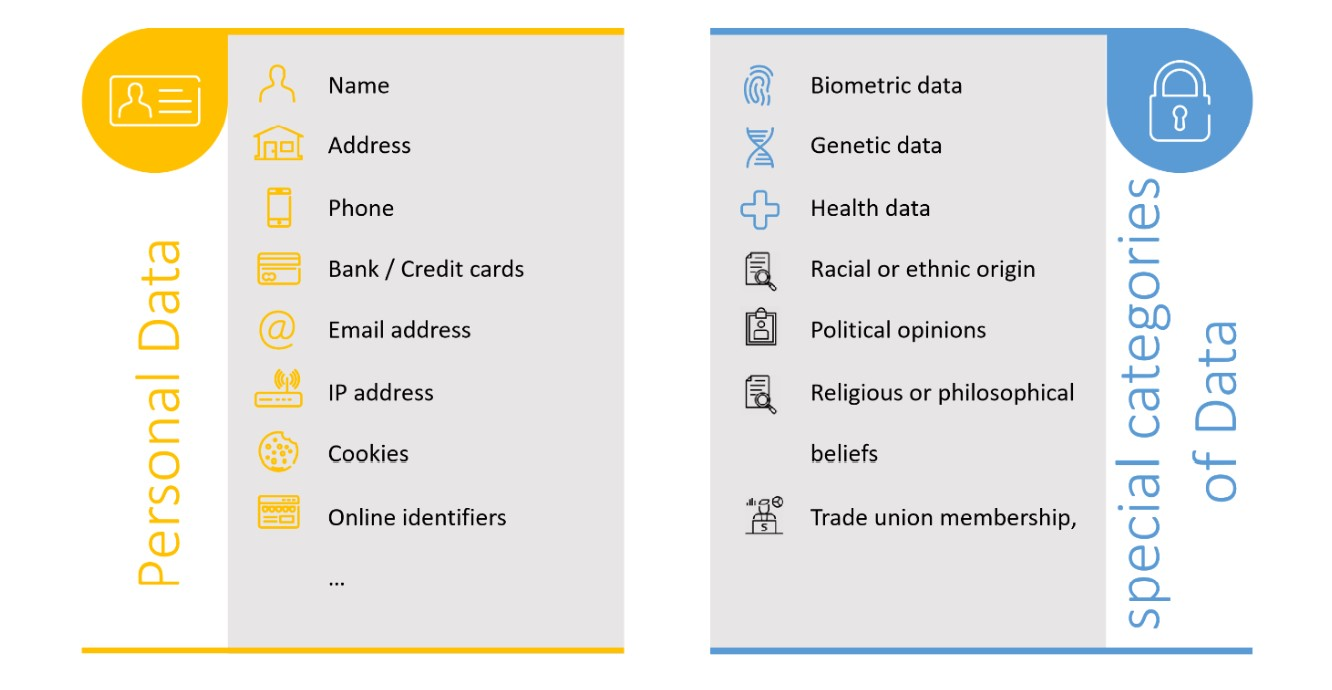
\includegraphics[width=12cm]{Images/personal data.jpg}
    \caption{type of personal data}
\end{figure}

Before GDPR, in its “Opinion 4/2007 on the concept of personal data”, the \textit{European Commission Article 29 Data Protection Working Party (WP)} clarified the notion of “personal data” with the idea that we can profile a person even if we don’t know its identity and, as a consequence, we are able to adapt some specific decisions about that person. Notice that all these issues about data protection don’t involve collecting data per se, but collecting data to make decisions which can affect the person.
Another debate was based on the \textbf{IP address}, which have been considered as protected personal data. Also in this case, the Working Party has considered IP addresses as data relating to an identifiable person, since Internet access providers can, using reasonable means, identify Internet users based on their attributed IP addresses using log files. IP Address is considered personal data also in GDPR.
Some peculiar examples are:
\begin{itemize}
    \item \textbf{Facial recognition systems} collect biometric information about individuals and in many cases these information are deleted but for a short moment it remains in the system so represents a sort of personal data processing.
    \item \textbf{Devices which collect voice} : voice is a feature of the individual so it’s a personal information.
    \item \textbf{Smart cities} are big and complicated environments with a lot of sensors with many information which reveal the behavior of many groups of people and individuals;
    \item \textbf{Wi-fi spectrum}: recent studies have demonstrated that in some conditions, the change of the shape of this spectrum, due to the movement of a body in an area, allows you to identify a person in a very precise manner.
\end{itemize}
So the notion of personal information in the current technological scenario is very broad because there are different technologies which are able to provide us a wide range of data and, by using them, we can infer information to identify a person.

To help us better understand where to start we have the \textbf{Recital 26}, which says "The principles of data protection should apply to any information concerning an identified or identifiable natural person, to determine whether a natural person is \textbf{identifiable}, account should be taken of all the \textbf{means reasonably likely} to be used, such as singling out, either by the controller or by another person to identify the natural person directly or indirectly. To ascertain whether means are reasonably likely to be used to identify the natural person, account should be taken of all objective factors, such as the \textbf{costs} of and the \textbf{amount of time} required for identification, taking into consideration the \textbf{available technology} at the time of the processing and technological \textbf{developments}."

\subsubsection{Reasonableness}
To assess the risk of re-identification (so elements which make possible to re-identify the individuals), we have to take into account:
\begin{itemize}
    \item \textbf{Cost of re-identification}: for example, if it’s very expensive to re-identify some information, it’s unlikely that this will happen;
    \item \textbf{Time}: if it takes a lot of time to re-identify, data is safer and will probably remain anonymous;
    \item \textbf{Available technology}: we have to consider the technology used for data processing;
    \item \textbf{Update the risk}: taking into account new technologies, for example something strong in terms of anonymization a few years ago can be very weak now because of new technologies which reduce the amount of money and time to re-identify.
\end{itemize}
There is also information about the use of \textbf{pseudonyms}, in particular they are still a part of GDPR, since persons can be identified using additional information.

\subsubsection{Anonymous data}
The last category of data cited in recital 26 is anonymous data, which is divided in two types:
\begin{itemize}
    \item Information that are anonymous since the origin (e.g counter in the streets that counts the number of cars).
    \item Information that have been anonymized (e.g personal information rendered anonymous by removing all identifiers)
\end{itemize}
Anonymous data is not part of GDPR. Might be difficult to achieve since there are no EU prescriptive standards for anonymization.

\subsubsection{Non-personal data}
There exists a regulation about non-personal data, but it's not part of GDPR. In particular, non-personal data can be defined as data that does not contain any information that can be used to identify a natural person. For example, all data shared between machines/robots in a smart industry context are not referred to individuals. Another example is the information about the level of pollution in a city or other information about the environment. There is free-flow of non-personal data.

\subsection{Article 5 - Main principles}
In the first part of the main principle we analyze lawfulness, fairness and transparency.
\subsubsection{Lawfulness,Fairness,Transparency}
\begin{itemize}
    \item \textbf{Lawfulness} refers to the compliance with the law; 
    \item \textbf{Fairness} means that you should process personal data in ways that people would reasonably expect and not use it in ways that can cause counter effects on them. For instance, if you are a patient in an hospital, some data are collected in order to provide you health care services. If this data is re-used for different purposes and/or you are not informed about that and/or the processing is not carried out in compliance with GDPR principles, this is an unfair use.
    \item \textbf{Transparency} means being clear, open and honest with people about who you are, how and why you use their personal data.
    Transparency plays a relevant role, not only in terms of information provided to the data subject when asking for consent, but, more in general, transparency is about the use of data and about the logic that underpin these systems that in many cases are not so clear.
\end{itemize}

\subsubsection{Purpose limitation}
Another principle is the purpose limitation principle, which says that "personal data can be collected for specified and legitimate purposes and not further processed in a manner that is incompatible with those principles. Further processing for archiving purposes in the public interest, scientific or historical research purposes or statistical purposes shall, in accordance with Article 89(1), not be considered to be incompatible with the initial purposes".
Furthermore, we can split this in:
\begin{itemize}
    \item At the moment in which you collect the data you have to clearly specify the purposes of data processing, what this means is that you cannot use a very generic and indefinite purpose, but you should be very specific in describing the purpose and explicit. Any further processing activity must be compatible with the original purpose.
    \item You can archive/process this data as long as it is used for public interest, scientific or historical research purposes or statistical purposes; these purposes are considered, by default, as compatible. If not, (in Italy) we can keep it only for 10 years from the end of the activity, then data needs to be destroyed. 
\end{itemize}

\subsubsection{Data minimisation}
You can collect and process personal data but, in doing that, you have to reduce at the minimum level possible data collection and processing. For this reason, article 5.1.c says that “data should be adequate, relevant and limited to what is necessary in relation to the purposes for which they are processed”. The use of data should be adequate and not excessive with regard to the purpose of data processing.

\subsubsection{Accuracy}
Accuracy means that data that you collect and process is correct and represent the facts described by this information. It must be kept up to date and any inaccuracy must be deleted or rectified, without delay, using any reasonable step. Accuracy is very important for both the data controller and the data subject for decision making:
\begin{itemize}
    \item Data controller, because it could take wrong decisions;
    \item Data subject, because wrong decisions can directly impact them;
\end{itemize}
Accuracy is strictly related to the process' purpose. For example, if you collect information for the purpose of providing credit, all the information that may have an impact on the decision to provide or not credit should be accurate. If you collect information for marketing purposes, the fact that they are not accurate is not relevant for the data processing concerning the credit (not relevant for that purpose) but are relevant to the processing activity concerning the marketing.
\subsubsection{Storage limitation}
Storage imitation means that you can collect information and use them for no longer than is necessary for the purposes that you have at the moment of data collection. The notion of necessity is something that cannot be measured in abstract but should be checked case by case. Data could be stored for longer periods solely for archiving purposes in the public interest, scientific or historical or statistical purposes
\subsubsection{Integrity and confidentiality}
It means security in terms of legitimate access to information, so only the person that are authorized to have access to the data should access to this information in order to preserve confidentiality and integrity.
\subsection{Accountability principle}
Accountability means being able to explain the decisions that have been taken about data processing step by step with ample documentation. The controller should be be responsible for and able to demonstrate compliance with the above principles. From a risk management perspective, it is not enough to put some safeguards, but it is also important to demonstrate what you have done. In other words, you can decide not to respect GDPR, but you should be able to demonstrate why.
\subsection{Data processing}
Any kind of operation on personal data is data processing. Data processing regarding a purely personal or household activity carried out by private individuals doesn't fall under GDPR. The four pillars of GDPR about data processing are the following:
\begin{itemize}
    \item Records of processing activities: each controller must maintain a record of processing activities to have an overview of what has been done with personal data, to know how much time to keep data or how much data the controller has. (Risk assessment);
    \item Data processors: when processing is to be carried out on behalf of the controller, for example tools that process data like Gmail, the processor must provide guarantees of technical and organisational measure. The controller and the processor must stipulate a Data Processing Agreement (DPA) to regulate personal data processing.
    \item DPIA (data protection impact assessment): When a process can lead to a high risk for the rights and freedom of data subjects the controller must provide an impact assessment on the protection of personal data before the processing begins. It's an expression of the accountability principle because the controller must demonstrate that the processing is compliant with the GDPR and how this is guaranteed.
    \item Data breach: After being aware of data breach the controller must notify the supervisory authority not later than 72 hours. It's useful to make others aware of threats and also because otherwise the company could never tell.
\end{itemize}
\subsubsection{Personal Data Processing Activities}
\begin{itemize}
    \item Lawfulness of data processing: processing of personal data is lawful if at least one of the following applies:
    \begin{itemize}
        \item Consent of the data subject;
        \item A contractual obligation;
        \item To satisfy a legal obligation.
        \item To protect the vital interests of the individual.
        \item To carry out a task that is in the public interest.
        \item For your company’s legitimate interests, but only after having checked that the fundamental rights and freedoms of the individual
    \end{itemize}
    \item Personal data relating criminal convictions (Article 10): shall be carried out only by the official authority or if authorized by the Union or by a member state law. The register of criminal convictions shall be kept only under the control of official authority.
    \item Processing of special categories of personal data (Article 9): 
    Special categories of personal data are personal data revealing racial origin, political opinions, religious beliefs, sexual orientations, genetic data, etc. All of this data is protected with a higher level of safeguards due to the fact that these data can be used for discrimination purposes and touch the personal spheres of individuals. 
    shall be lawful only if one of the following applies:
    \begin{itemize}
        \item The consent of the individual concerned
        \item Processing is necessary for social security and social protection law
        \item Processing is necessary to protect the vital interests of the data subject
        \item Processing carried out in the course of its activities by a foundation, association or any other not-for-profit body
        \item Personal data which are manifestly made public by the data subject
        \item Processing is necessary for the exercise or defence of legal claims
        \item Processing is necessary for reasons of substantial public interest. There must be a balance between the risk for society on one hand and the impact on individual rights on the other hand. Some measures to reduce this impact can be taken such as limiting access to this data only to specific individuals or deletion after some time, etc.
        \item Processing is necessary for the purposes of preventive or occupational medicine
    \end{itemize}
    In this case consent is enough.
\end{itemize}

\subsection{Article 7 (Consent)}
Consent: the consent is the best expression of the self-determination of individuals, so according to the traditional idea of data protection as a form of control of personal information, consent is one of the main pillars in terms of the legitimacy of data processing.
Article 7 describes the manner in which consent can be collected:
\begin{itemize}
    \item \textbf{consent should be informed}: some specific pieces of information must be provided to the data subject, and so the data subject can give consent to data protection for one or more specific purposes.
    \item Be able to \textbf{demonstrate} that the data subject has consented, which is in line with the concept of accountability;the process in which the consent is collected must be documented.
    \item In a written declaration, the consent should be \textbf{freely expressed} and \textbf{distinguishable} from the rest of the different agreements between the data subject and the controller: so in a contract (or other agreements), the consent for different purposes are stated separately. Moreover, the consent should be intelligible and easily accessible form, using clear and plain language.
    \item  Situations in which personal information are acquired by contract, although they are not relevant for the contract itself, such as when the data subject is required to fill a form with many data that are not relevant for the purpose of data processing. This is an unfair bargain and it is not possible to collect the data if they are not necessary for the provision of the service.
    \item Imbalance: consent is not freely given in imbalanced situations, considering both private and public sectors, such as a public authority which has power over citizens: consent can not be a legal ground (excluding limited situations), public authorities process data according to specific provisions of the law so they do not need consent as a legal ground, there is another legal ground that authorizes such processing.
    \item The right to \textbf{withdraw}: if there is consent since it is an expression of self-determination, it is considered as a unilateral act, so the data subject is always able to withdraw it.There are some challenges in AI because in AI I can withdraw consent to train a machine, but the problem is that, although personal information is deleted from the dataset, the trained machine is still able to identify you because it already learned it.
    \item \textbf{Consent provided by minors}: the threshold in GDPR to provide autonomous consent is 16 years old, but there is this provision that gives a range from 13 to 16.
\end{itemize}

\subsubsection{Other legal grounds}
In this section are present some cases in which is not mandatory have the consent.
\begin{itemize}
    \item Compliance with a legal obligation: the EU laws or national laws ask you to process personal information. E.g. online service providers that detect infringement of criminal laws, in certain circumstances the provider has to communicate user data to the authorities according to this legal ground, which is compliance with a legal obligation (a law ask you to do that), consent of the data subject is not required.
    \item The data subject is not able to provide the consent and the data processing is necessary to protect the data subject, such as vital interests of the data subject. E.g. processing of health data in first aid service: the data subject, due to their conditions, is not able to provide consent, but their information is needed in order to provide first aid: this situation is covered by this legal ground.
    \item Public interest: when there is a public interest of the society, any other legal grounds or data subject consent are not needed.. E.g. Public health.
    \item Legitimate interest concerns the interest of the entity that processes the data (the data controller) in carrying out specific activities related to data processing.  E.g. some marketing purpose activities are consistent with the nature of the product that was sold to the client, such a commercial offer regarding spare parts of the car that should be changed after some time: this is legitimate interest because it is a legitimate interest of the company to provide a good service to the client. Legitimate interest requires a balancing test: this is a legal ground unless some interests are overridden, which are fundamental rights and freedoms of the data subject regarding the protection of personal data.
\end{itemize}


\subsubsection{Case Study}
Claudia orders a pizza via a mobile app on her smartphone but does not opt-out of marketing on the website. Her address and credit card details are stored for the delivery. A few days later Claudia receives discount coupons for similar products [legitimate interest,impact] from the pizza chain in her letterbox at home [impact].\\
There is a legitimate interest in providing discounts to attract clients to use the service, and there is lawful interest, there is an impact on the data subject but it is quite limited, there are safeguards because the client can opt-out from receiving such coupons.\\
\textbf{In this example, legitimate interest prevails over data protection because the legitimate interest in promoting the business prevails since the data about the user is very limited and not sensible, and also the negative impact is limited}.

\subsection{Main Characters}
The GDPR has a procedure approach, this means that since the moment in which we collect the data, to the end in which we destroy data or transmit it to third parts, there are different kinds of person that may interact with personal information. This means that data processing is not something that is put in practice by one person only. Usually data processing activities are carried out by companies, involve different kind of branches, and in some special case there is also an interaction with third parties like other entities or companies that provide services.

In this sense the main distinction is between \textbf{data controller} and \textbf{data processors}. The main idea is that there is a sort of pyramid of the rule and relationship of the people that carry out data processing activities. At the top of this pyramid there is someone that decide the purpose and the technical solution to process this data, and then at lower level there are other people that have a really limited impact on the structure of data processing, they just carry out minor activities of data entry.

In this sense there is someone that has the power to decide which is the target, the purpose of data processing , This rule is covered by the data controller. Than there is data processors that cooperate with the data controller but he is not able to fully shape the data processing but act in the aim of the controller.
\subsubsection{Data controller} 
In this sense the controller is defined by the GDPR as the natural or legal person, public authority, agency or other body which,alone or jointly with others, \textbf{determines the purposes and means of the processing} of personal data. According to the GDPR rule, if you are the controller you are the person that is able to have a direct impact on which data you want to collect, for which purpose and can't use this data for a purpose that is different from the purpose that has been decided according to the law and the data subject. For this reason a bank, for example, usually chooses the bank itself as data controller, because it has a huge power and at the end of the day it cannot be in the hand of a single person. (L'ho messo perchè fa molto:"da grandi poteri, derivano grandi responsabilità"). It is possible have two or more controllers and in this case It’s important to define a formal agreement between \textbf{joint-controllers}: is important to define who has the control during different kind of data processing activities. So who is liable and accountable for every different purpose.
\subsubsection{Data processor}
Processor is a natural or legal person, public authority, agency or other body which \textbf{processes personal data on behalf of the controller}. This means that the processors carry out the processing activities, in many case concretely deciding the manner, the security aspect and etc... but always on behalf of the controller. So this is the main distinction between processor and controller: the processor analyses data but not for his own interest. You can be a data processor and a data controller at the same time.
\subsubsection{Sub Processor}
The sub processor is described as third figure that carries out part of the activity that the controller assigned to the processor. The processor can engage another processor with prior specific or general written authorisation of the controller (Article 28.2). It means that if you are a processor you cannot decide autonomously to engage a sub-processor, you have to concord this with the data controller. Because the controller is liable for both and so must have the chance to check in terms quality, in terms of skills who is going to take part to the data processing activity. This authorization can be specific: the controller decides who can be the sub processor and so the controller maintain the full control on the data processing activity.
\subsubsection{Data subject}
The Data Subject is the identified or identifiable natural person [s] owner of the data provided. The GDPR formally assigns five fundamental rights to the Data Subject:
\begin{itemize}
    \item right of access: the data subject has the right to know which of the data he has provided will be used by the controller and for what purpose. The data subject has the right to request a copy of this data that the controller must provide (also remotely);
    \item right to be forgotten: the data subject must always be able to delete the data concerning him;
    \item right of rectification: the data subject has the right to request the modification of their data;
    \item right of limitation: the data subject may request the limitation of the use of data where, for example, the data is incorrect;
    \item right to data portability: the data subject has the right to obtain the data provided to the controller in a structured and readable format. In response to the request, the controller must provide the data to the user within one month, a period that can be extended to three months in particularly complex cases, provided that the data subject is informed of the reasons for the extension. The data subject may decide to transmit such data to another controller.
\end{itemize}
\subsubsection{Data protection officer}
DPO is an expert in data protection laws and GDPR that understands operations performed on data and the technologies used. The DPO has a an overview of all the processing activities and assures that everything is compliant with the GDPR. It would be good practice to always have a DPO but it's mandatory in the following cases:
\begin{itemize}
    \item Public authorities or bodies: a single data protection officer may be designated for several authorities/bodies.
    \item  DC/DP that regularly and systematically monitor data subjects on a large scale.
    \item  DC/DP that process on a large scale special categories of data or personal data relating to criminal convictions and offences.
\end{itemize}
It's important that the DPO has enough resources to carry out its taks independently, in particular the controller should not interfere with his work or give penalization based on its performances. There must be no conflict of interest with other tasks and duties.
DPOs are not personally responsible for non-compliance with data protection requirements (data protection compliance is the responsibility of DC/DP). It is not liable, he just make suggestion and if the DC decide for other strategy, just the controller is liable.
\subsection{Accountability}
The decision-making power over data processing and the diferent accountability/liability is the criterion for distinguishing between controller/processor. 
\begin{itemize}
    \item The \textbf{data controller} has the total control over the data processing but is also liable and accountable for the activity. If the company qualifies as the controller, but is not able to shape/define the purpose of the processing activity, the fact that is qualified as the controller is irrelevant.
    \item The \textbf{data processor} has no control over the data processing but it's not liable for the decisions adopted by the data processor. It could be liable if the decisions and the guidelines of the data controller are not respected. The processor must provide sufficient guarantees to implement appropriate technical and organisational measures in such a manner that processing will meet the requirements of the GDPR (Article 28.1).
\end{itemize}
Contractual relationship between controller and processor are defined in Article 28.3. The contract should set:
\begin{itemize}
    \item the subject-matter and duration of the processing.
    \item the nature and purpose of the processing.
    \item the type of personal data and categories of data subjects.
    \item the obligations and rights of the controller.
\end{itemize}
It could happen that the the data controller chooses the data processor in another country where the data protection law is different and maybe less secure. In this case it's necessary that between the data controller and data processor is adopted an agreement to make clear the role of each entity involved in data processing and so who must be liable and accountable at each phase of data processing.

Usually the data controller can be compliant about:
\begin{itemize}
    \item Security measures.
    \item Risk management.
\end{itemize}

There is not a list of things that each entity can do in order to prevent issues and personal data violation, but there are only principle or suggestion in the GDPR. To partially simplify the accountability certification there is the introduction of some form of codes of conduct, certifications, seals and marks. 

Another important thing to assure accountability is to adopt a data protection strategy, to identify weaknesses and priorities.
The steps are:
\begin{itemize}
    \item Map the data flows and processing activities. This is useful because you might find that some aspects are not completely known and it could be difficult to assure data protection.
    \item Map task distribution. In this way you know exactly who is involved and for what. 
    \item Finally evaluate all the potential risks and define procedural and technical measure to reduce them.
\end{itemize}
\subsection{Security and risk assessment}
\subsubsection{Data Security}
With the objective of protecting the data subjects privacy, one of the best approaches is to have applications designed with privacy in mind.
Our focus is on personal data, to avoid the negative consequences of its use. This is strictly correlated to fundamental rights.
Using personal information, you can affect freedom of movement and freedom of speech, so we have to consider the consequences of data processing in terms of rights and freedom.
Security mainly deals with the protection of the information, and it's easier to be monitored and managed (the risk is easy to understand). Measures have to be adopted to guarantee a security level comparable to the risk of illicit access to data. For example:
\begin{itemize}
    \item A bank account has a high financial risk, that can be reduced by assessing the high risk, which is more or less measurable, and adopting the necessary measures. 
    \item In a smart city plan, there are potential negative consequences on the citizens in terms of data protection and rights, since someone could have access to data about mobility, use of social networks, smart devices at home etc.
\end{itemize}
Data security is the first stage of the risk assessment and is focused on the traditional idea of risk from a computer scientist perspective.
\subsubsection{Security measure}
Article 32 of the GDPR focuses on security measures and obligations that both the data controller and data processor have to comply to in order to perform data processing. Despite the controller being the one that defines the strategy, the data processor still has to adopt measures in terms of data security while also being compliant with the controller's instructions. Both controller and processor also have to supervise other parties, that means every person involved in data processing should follow the instructions provided by the controller/processor. The only exception is represented by the case in which there are specific legal provisions required to process data in a certain manner.

Regarding accountability, the two main parameters we have to consider in verifying it are the \textbf{likelihood} and the \textbf{severity} of the risk. For example:
\begin{itemize}
    \item A breach to a bank account has a negative impact on the right of property;
    \item A breach to a social media account has a negative impact on the right of privacy.
\end{itemize}
To tackle this kind of risks we have to consider \textbf{two stages}:
\begin{itemize}
    \item The first stage is the \textbf{risk assessment}, assessing the likelihood and the impact of potential negative consequences of a breach of security;
    \item The second is the \textbf{adoption of the measures to tackle this risk}, that should be appropriate to the risk.
\end{itemize}
There are different types of security measures:
\begin{itemize}
    \item technical: computer-based or technology-based for example a  firewall, use of encrypted data etc.
    \item organizational: measures that concern the staff that is involved in processing information, for example limit the access to sensitive information only to certain employees.
\end{itemize}
These measures should be adequate to tackle the risk, so we consider several parameters:
\begin{itemize}
    \item The nature of data processing: Different kinds of potential impact are related to the nature of data that is processed, so we have to consider the scope of data processing. For instance, processing information in order to provide market information or to recruit people are different things.
    \item Context: The situation in which you process personal data, for instance, if you are carrying out an emergency action as red cross there is a risk of hacking or other negative impacts on data processing. The risk is for rights and freedom.
    \item State of art and cost of implementation: To provide adequate safeguard to the personal information we have to maintain as a key element the notion of proportionality. For example you can use a satellite control to prevent any access to your office, but if in your office you have very basic and inoffensive personal information this is not necessary, it's enough to lock the door. On the other hand, it's also important to consider the \textbf{state of the art}. If you lock information inside an encrypted file, you have to consider the strongness of the encrypted solution that you have adopted over the years, because with the progress of technology, what was safe and secure in the past may no longer provide the same level of security in the future.
\end{itemize}
For this reason, the GDPR provides some examples in terms of technical solutions, but it's an open list since over the years technology may change.

The GDPR decides not to provide a \textbf{minimum standard} but to adopt a risk management approach, because the minimum level can be high in some cases when data processing is basic and the risk is very low. This increases the level of freedom and at the same time the level of accountability, because as a controller/processor you have to assess the risk and select the measure that is adequate to tackle that risk.

In this sense the article on security provides only some examples of potential solutions:
\begin{itemize}
    \item pseudonymization: as described in art. 4 of GDPR, it means to remove (but not to delete) the identifiers of personal data, so  the dataset is split: one dataset is without identifiers, but using for instance hash, we can match this dataset with another dataset in which there are the identifiers;
    \item encryption of personal data: encrypted data remains personal data. If you are able to destroy all the keys, data is no longer personal;
    \item general reference to measure for confidential integrity,like encryption and firewall;
    \item measure to ensure availability, business continuity and resilience: resilience is an important aspect because security means to maintain a system in a manner that is efficient and can provide the service. So, continuity is very important because without it there is a risk not to have access to data, not to process it, and this negatively affects individuals.;
    \item testing tools;
\end{itemize}
As we have mentioned the fact that the technology contest is in continuous changing, also the measures should be periodically reviewed and updated taking into account the new challenges and threats in term of data security.

\subsection{Key aspects of security and data protection}
There is a table contains the provisions of the GDPR and the key aspects in terms of security and in terms of security data protection.
\begin{figure}[!h]
    \centering
    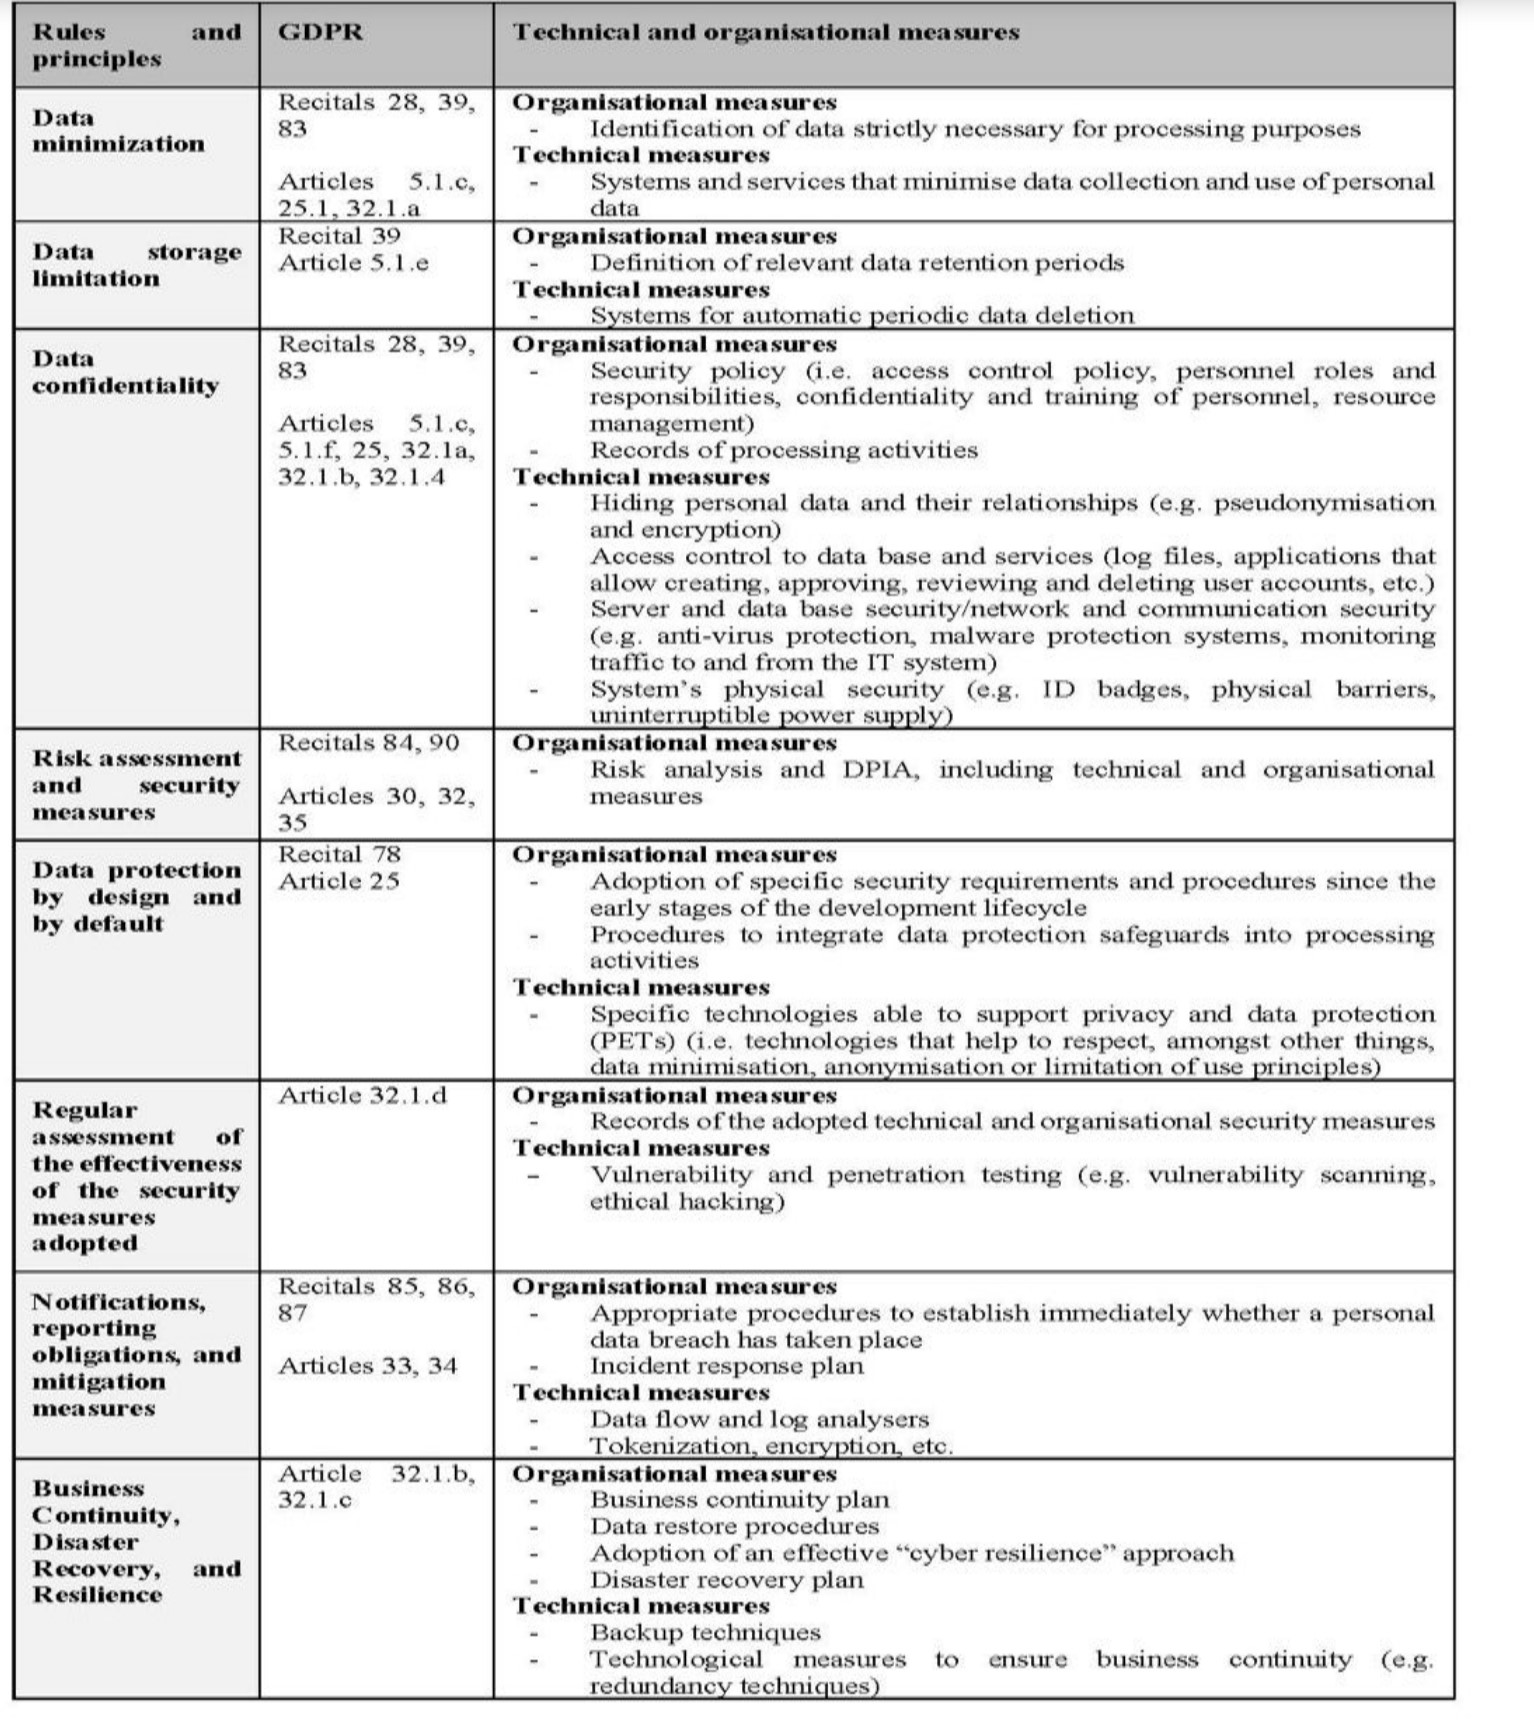
\includegraphics[width=12cm]{Images/Table security.jpg}
    \caption{Table security}
    
\end{figure}
Another idea of this table is that there are also some measures concerning notification and reporting activity because as we see in case of a data breach, there are specific mandatory requirements in order to make aware the data protection authorities and in some cases also the users of the data breach (in 72 hours). 

Business continuity plan and data store procedures are all aspects concerning resilience or better cyber resilience, that is something that has to be considered to tackle these security risks.This table is important to give a sort of an overview about how this general principles that we found on the GDPR, concerning risk management and security, could be and should be detailed in some specific measure in terms of organization of the strategy that you have in your company or public body and in terms of the technical measures that you can use for this purpose.
\subsection{Risk Management and DPIA}
DPIA is “Data Protection Impact Assessment” and refers to the procedure that is explicitly required in some case by \textbf{Article 35} of the GDPR. In the GDPR as in data protection history, risk management is a key point, but what is new in the GDPR is that we have a sort of definition of the procedures that we have to adopt in terms of risk management in the field of data processing.
\subsubsection{A three-step strategy}
We can describe DPIA as a three layers strategy:
\begin{itemize}
    \item \textbf{Preliminary analysis}, ex-ante component: necessary to carry out the data strategy. We define for example how to manage and collect data, that is which kind of data, what are the purposes, the data flow, etc.
    \item \textbf{Data strategy and data management}, the core component;
    \item \textbf{Data minimization and by-design approach}, the ex-post component: here we put in practice the measures.
\end{itemize}
\subsubsection{Preliminary analysis}
The first step is the preliminary analysis, and this is specifically required by \textbf{Article 30} of the GDPR, in which both data controller and processor are required to carry out a sort of map of the data flows. It is not mandatory if you process data in a company with less than 250 members unless the processing is likely to result in a risk to the rights or freedom of data subjects or in the case in which the process includes special category of data.
Example of map of data flows:
\begin{itemize}
    \item \textbf{Categories of the data subject and of personal data} is something that is important for the controller, that has a general overview of the process and that is directly accountable with regard to the data subject. It is also true that this is a piece of important information for the data processor because different categories entail different kinds of standards in terms of security and risk management.
    \item The \textbf{category recipients} follow the same indications, so is the controller that decides which kind of entity can receive the information.
    \item The \textbf{transfer to a third country or an international organization} is an activity that can be carried out by both, so they should be both aware about the legal constraints that are related to the transport, mainly this data moves to Europe to a European country.
    \item The \textbf{estimated time limits for erasure}, i.e. the retention for different kind of data, this again is something that is part of a general strategy of data processing, again is the controller that should collect this information
    \item The \textbf{description of technical and organizational security measures} is an obligation that concern both the controller and the processor because, although the processor processes the data on behalf of the controller, the processor must necessarily adopt the security measures that are required by the specific context.
\end{itemize}

This sort of map is important for the company that carries out the processing activity, but is also important in terms of accountability (allows for identification of various components in the processing of data). This step is not mandatory but it's likely to happen anyway, since it is very important in case of inspection.

Preliminary analysis was the first step. On the basis of this monitoring activity, you now are aware of the data flows that you have inside and also of the relationship between your entity and the data and between your entity and third parties that are involved in data processing.
\subsubsection{Risk assessment and management}
Risk assessment means that you have to check the different processing activity that you carry out, and for them consider the potential risks involved.
It's important to consider the granularity, because if you have a long list of processing activities split it into many sub-processing activities, in case of big data flows, the risk is that you may end up with hundreds of processing activity.
The risk assessment based on the flows of information that you have collected is a self-assessment. As a controller or as a processor you have to assess the risk, case by case, that some processing activity may have for the individuals that are involved. Note that the risk is a risk in terms of impact on individual rights and freedoms, so how the processing of information may negatively impact on privacy, data protection, freedom of speech, freedom of movement or any kind of right that could negatively be affected by the use of this data.

There is a first \textbf{general assessment} (Sect. \ref{sect:general_assess}) , then there is a \textbf{formal assessment} (Sect. \ref{sect:formal_assess} \ref{sect:DPIA}), then the \textbf{prior consultation} (Sect. \ref{sect:prior_cons}), and then a general compliance and enforcement is carried out according to GDPR provisions. If you do not follow the mandatory requirement in terms of risk assessment that are in the GDPR, there are high sanctions (Art. 83), that are up to 2 \% of the total worldwide annual turnover. Formal assessment is required only when there is a high risk.

What is important to consider is that in any case you always have to carry out an impact assessment (DPIA), then when you realize that the risk is high, the impact assessment will be formalized using a formal document, according to the standard provided by GDPR and IDP. The distinction is only between the case in which, due to the fact there is a high risk, this impact assessment should be formalized and put on paper, while when the impact is low-medium, the law does not ask you to provide this document, but it's still better to have it.
\subsubsection{General assessment}
\label{sect:general_assess}
The controller and the processor shall implement appropriate technical and organisational measures to ensure a level of security \textbf{appropriate to the risk}. These measures are based on the state of the art and the cost of implementation. Since the technology and the risk may change, you are required in many cases to carry out the risk assessment after some time (6 months, 1 year, 3 years,…), it depends by the technology and it depends by the change in the nature of the risk and the threats.
\subsubsection{Circular approach}
\begin{figure}[!h]
    \centering
    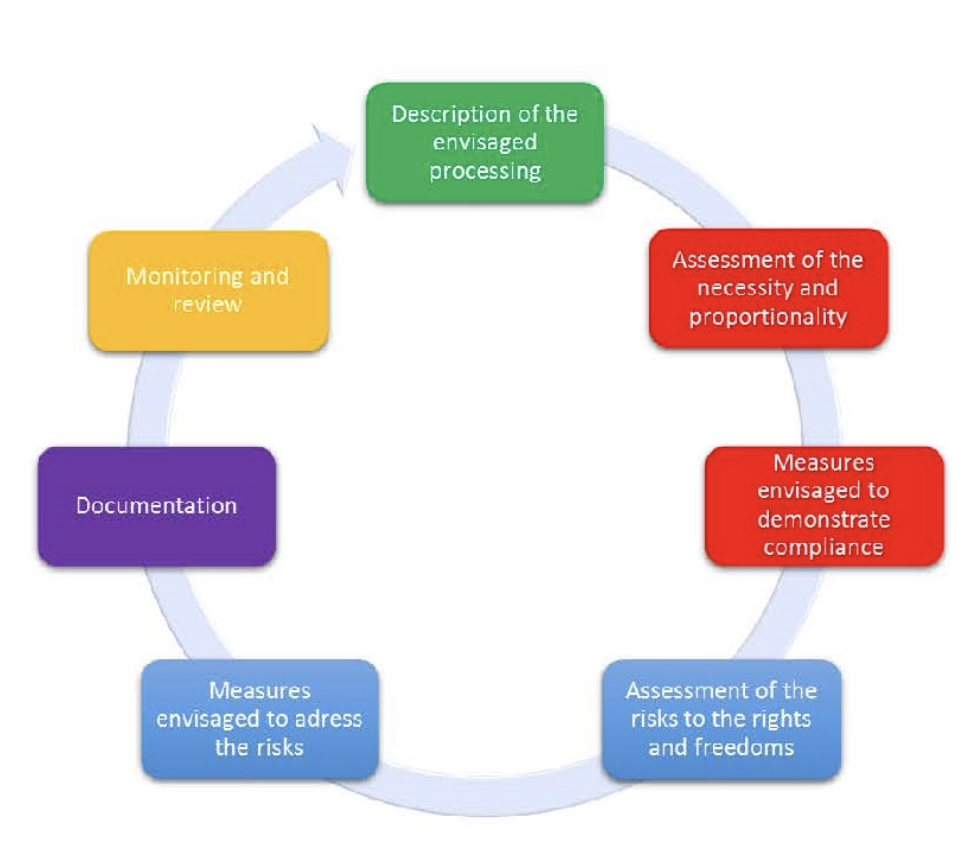
\includegraphics[scale=0.6]{Images/Circular Approach.jpg}
    \caption{Circular approach}
    \label{fig:circular_approach}
\end{figure}
The steps in Fig. \ref{fig:circular_approach} are:
\begin{itemize}
    \item purposes of data processing, that is the same for both entities. Because in both the cases if you monitor data flows, although you process data on behalf of another entity, you have to know the purpose of data processing to understand the potential risk etc.
    \item monitoring of activities (description of the envisaged processing)
    \item assessment of the risk, in terms of the necessity of processing activities and proportionality
    \item measures to avoid any excessive collection of data or invasive data processing activity
    \item assessment of risk, in terms of rights and freedoms
    \item measures adopted to tackle the risk
    \item documentation, that is the formal impact assessment (used also in the case of low or medium risk)
    \item periodical monitoring in order to assess if the risks are changed (they can increase, decrease, new risks may arise) and if the measures are adequate or no longer adequate
\end{itemize}
This circle is the same also in the hypothesis in which the risk is high because it follows the same approach. The distinction is on the documentation because in the case of a high risk you have to prepare a specific document, that is\textbf{ Data Protection Impact Assessment} (DPIA), a detailed description of your risks and the measures used to tackle them.
\subsubsection{Formal assessment}
\label{sect:formal_assess}
It's the DPIA. The formal assessment is described in the art. 35 of the GDPR. The general rule is that this is required only when there is a high risk. But this general provision is useful because it may include situations that we do not know or that we are not able to predict at the moment in which you write the text of the law. These situations of high risk are \textbf{presumptions}, which means that the legislator, based on what normally happens, consider that these situations exist, even though there is no evidence.
In particular it is required if:
\begin{itemize}
    \item the company executes automatic evaluations of personal aspects relating to natural persons (profiling). If there are mistakes in decision making they may affect the livelihood of the data subject.
    \item processing on a large scale of special categories of data or of personal data relating to criminal convictions and offences;
    \item a systematic monitoring of a publicly accessible area on a large scale.
\end{itemize}
\subsection{DPIA (Data Protection Impact Assessment) - By design approach}
\label{sect:DPIA}
By design approach means to consider the impact on data protection of a processing \textbf{before} starting the proceeding itself, and reshape the processing acordingly. 
This is in contrast of the by default approach, that means to protect by default only  necessary personal data for each specific purpose.
To make a risk assessment, you need to describe what you assess:
\begin{enumerate}
    \item A systematic description of the envisaged processing operations and the purposes of the processing, including, where applicable, the legitimate interest pursued by the controller. DPIA is not something you carry out at the end when all the processes are defined and the services/products are already shaped but is something that starts from the beginning. Every time that you add something new in the product, you have to check the consequences on data protection and you have to redefine your assessment. 
    \item An assessment of the necessity and proportionality of processing operations in relation to their purposes: that means that you need a reason to collect specific data from the data subject which should be related to the purpose of the application.
    Note that you can decide to collect data not strictly related to the main purpose of the app but for some other specific purpose, but strictly on the base of the agreement with the data subject.
    \item The assessment of the risks to the rights and freedoms of the data subjects
    \item The measures envisaged addressing the risks, including safeguards, security measures and mechanisms to ensure the protection of personal data and to demonstrate the compliance with the GDPR.
\end{enumerate}
This document is quite easy in terms of structure because, the difficult part is the assessment of a risk.

\subsubsection{DPIA Nature}
In terms of structure, DPIA is a question-based assessment. Usually there is a list of questions that drive the data gatherer in understanding the key elements and related risk of the processing activity.
It is a context-based analysis, in fact it is based on the specific activities that we are monitoring and we are assessing. There is a distinction between the part of impact assessment and the part about the potential impact on rights/freedom.

A plausible \textbf{approach} in writing a DPIA is:
\begin{itemize}
    \item It's important that the impact assessment, mainly when about a large scale project, have an interdisciplinary team;
    \item The analysis should start since the inception of the project;
    \item When the project is finished and we also have a final version of the impact assessment, the DPIA should be updated on the basis of any kind of elements that can change its parameters that have been considered to carry out this assessment (periodic verifications).
\end{itemize}

Another important point is that the DPIA can be also carried out by the manufacturer or the service provider. Who provides a service can also provide an impact assessment for this service.

The DPIA can be carried out not only for one specific processing activity but also for different processing activities that have similarities in terms of nature, purpose, risk, or context etc.

The last point, is that the DPIA should not be publicly available. It should be available to the Data Protection Authorities, in terms of accountability, but there is not any requirement for having a public available impact assessment.
A document with more details about the issues that are more challenging, from a
competitive and security perspective, and another publicly available part, will be probably a solution that could help data subjects to be aware of the risks of the use of the data. The availability of this document is very important to understand the risk of the processing activity, and this is more relevant in the case of data-intensive applications like data analytics and artificial intelligence.
\subsubsection{Data protection by default}
Practically it means that if you create a system, all the option concerning personal data should be set on "off", in a manner not to collect personal data, of course, if data are not necessary for the purposes of the software itself. This is the idea of privacy by default: when you create something, the default settings of this product should be privacy-oriented, it means collect less data as possible or completely anonymize.
Both by design and by default give us a clear message: if you create something that potentially has an impact on personal data, first you have to check if you can reach the same goal without using personal data and if you need personal data, you have to minimize and reduce the number of data that you collect. The idea is not only to reduce collected data but also adequately protect data and reduce the potential negative impact and risk of data processing.
\subsubsection{Prior consultation}
\label{sect:prior_cons}
In some cases, it may happen that, after DPIA, you realize that, although you adopt some specific measures, these are not enough. They are not adequate in terms of reducing the risk and it remains high.
For this reason, the GDPR introduced this idea of prior consultation. When you reduced part of the risk but there is still a margin of high risk, the solution is to ask to a Data Protection Authority, or Supervisory Authority, a prior consultation. It can happen for many reasons:
\begin{itemize}
    \item The complexity and the risk of the situation: the data authority can check the system and suggest some measures that maybe were not considered in the design of the product or suggest some changes to reduce the impact behind the threshold of high risk;
    \item the processing activity is an activity with a high impact and there is no remedy: This activity is against the law (the GDPR) and the Data Protection Authorities have no instruments to reduce this risk. The decision will be to stop this kind of activity.
    \item although there is a high risk in terms of data protection, the balance of interests can justify some limitation to privacy in data protection, for example the body scanner.
\end{itemize}
\subsection{Data Breach}
\subsubsection{Definition of data breach}
The definition of data breach is provided by article 4, like all the definition we have in GDPR. Data breach is defined as: \textit{“a breach of security leading to the accidental or unlawful destruction, loss, alteration, unauthorized disclosure of, or access to, personal data transmitted, stored or otherwise processed”}. A security breach can be:
\begin{itemize}
    \item accidental: for example, an employee sends personal data by mistake to someone who wasn't supposed to receive that data;
    \item unlawful: for example a hack to the IT system of a company.
\end{itemize}
There are different classifications of personal data breaches:
\begin{itemize}
    \item \textbf{Confidentiality breach}: abusive access to personal information. This affects confidentiality since this information should be accessed only by the controller, the processor or authorized people who work for them.
    \item \textbf{Integrity breach}: when there is the alteration of data. Some data have been changed due to a not legitimized access by a third party or individual.
    \item \textbf{Availability breach}: an accidental or unauthorised loss of access to, or destruction of, personal data.
\end{itemize}
\subsubsection{Obligations (Art.33)}
The GDPR specifies some specific obligations for controllers and processors in terms of quick reaction and adoption of a specific strategy to address a potential data breach. 
The Controller has to notify the data breach to the competent SA, taking into account the nation in which it has its headquarters. It is very important that this notification arrives on time, because the supervisor has to be aware of the state and the condition of this threat that is potentially high risk for data subjects. In this sense GDPR fixed a time limit for the notification of \textbf{72 hours} after the moment in which the controller has become aware of the data breach. However, this threshold can be extended providing an adequate motivation. Possible motivations usually are the fact that it is not clear the dimension of the breach, or which kind of data have been affected, so you do not have adequate information. 

The notification is not required when it is useless, so for instance when the personal data breach has not an impact on the rights and freedom of data subjects. In this case there are some protection measures that limit or make impossible any kind of negative effects.

\textbf{Accountability}: It is important to have a register of notifications and data breach events with details in terms of facts and the remedies that have been adopted in order to tackle the risk of this event (Art. 33.5). It is important to be able to show, in case of inspections, the level of compliance and, in the case in which you have not notified to the SA, to show that that breach was not relevant. Anything should be demonstrated and for this reason you need a data breach register, for which there are two tools:
\begin{itemize}
    \item incident log: concise but comprehensive and updated in a timely manner;
    \item internal reports: with standard and easily accessible templates, updated as action plans evolve with detailed risk assessment and documentation of decisions made within the organization.
\end{itemize}

\textbf{Data Processors}: When a breach happens to the processor, the duty in terms of notification is not to notify to the SA but the controller without undue delay, because it is the controller that has the general overview of the processing activity and should decide which kind of measure to adopt. The controller will see the notification, check if measures can be adopted or not and if there are potential risk for the rights and freedom of data subjects. It's still the controller that notifies the fact to the supervisory authority.

\subsubsection{Notification to SA}
The notification to the supervising authority has a predefined form and is composed of:
\begin{itemize}
    \item Name and contact details of the DPO/other contact point
    \item Description of the dimension of the breach and of the related risk, also in terms of sensitive data (nature of data, number of records affected, number of data subjects affected,..)
    \item Likely consequences of the breach
    \item Measures taken or proposed to be taken by the controller.
\end{itemize}


\subsubsection{Notification to Data Subject and Exceptions}
This happen only in the case in which there is a high risk to the rights and freedoms of natural persons. The content of the notification to the data subject is similar to the content of the notification to the SA, so you have to describe which kind of impact this breach may have for the data subject and which kind of measures you imagine adopting (both technical measures (ex. encryption, etc.) and organizational ones) in the future hours or days in order to minimize this impact.

There are some cases in which there is not the need to notify:
\begin{itemize}
    \item there is no risk;
    \item the breach does not include personal data;
    \item the controller implemente appropriate technical and organiational measures. The final decision is still made by the DPA that can impose the notification and sanction the controller;
    \item when the holder has taken measures to prevent high risks to freedom and rights;
    \item when the efforts to communicate would require disproportionate efforts, so it can be replaced by a public communication.
\end{itemize}

\subsubsection{Organizational Measures}
What is important in terms of accountability and risk management is to prevent this event, to end it, and/or to create an adequate solution to limit the potential effect of this negative event. It is important to have, according to the approach of GDPR, some specific procedure to address these challenges. For this reason, there are two main important documents to have:
\begin{itemize}
    \item \textbf{the notification procedure}: a sort of flow that describes who have to handle this kind of situations and the internal organization that have to address this challenge, because in many case you have to react in a very short time and so everything should be already defined like in a risk management situation.
    \item \textbf{incident identification system} and related \textbf{incident response plan} because you should be aware of the data breach. If you are not aware and you don’t have the technical system that detect some infringement in the protection of the data, you could become aware of the fact many months after. This is not a fair manner to process personal information, so it’s a source of liability.
\end{itemize}
You should define \textbf{roles and responsibilities} by involving primarily affected business functions (including CEO). In particular:
\begin{itemize}
    \item perform periodic simulations and program updates;
    \item be concrete and effective;
    \item detail how you will interact with the authorities.
\end{itemize}

To reduce the risks:
\begin{itemize}
    \item training and awareness raising;
    \item improve security measures.
\end{itemize}

\subsubsection{After a data breach}
The consequences of a data breach are:
\begin{itemize}
    \item direct loss of data or money;
    \item customer turnover;
    \item reputational and image damage;
    \item set up help desks;
    \item restore the information system;
    \item legal expenses and internal investigations.
\end{itemize}
The \textbf{remediation plan} is:
\begin{itemize}
    \item Correct the vulnerability that allowed the incident to occur;
    \item Improve your approach to information security;
    \item Share information with relevant stakeholders;
    \item Reinforce training if human error was the cause.
\end{itemize}
